\documentclass[12pt,a4paper]{article}

\usepackage{polyglossia}
\usepackage{microtype}
\usepackage[margin=1in]{geometry}
\usepackage{graphicx}

\setdefaultlanguage{ukrainian}
\setotherlanguage{english}
\setmainfont[Ligatures=TeX]{Liberation Serif}
\setsansfont{Liberation Sans}
\setmonofont{Liberation Mono}

\begin{document}
\begin{titlepage}
	{\centering
	\Large НАЦІОНАЛЬНИЙ ТЕХНІЧНИЙ УНІВЕРСИТЕТ УКРАЇНИ\par
	\large «Київський політехнічний інститут імені Ігоря Сікорського»\par
	\vspace{1cm}
	Кафедра програмного забезпечення комп'ютерних систем\par
	\vspace{1cm}
	\normalsize Лабораторна робота \textnumero1\par
	із дисципліни «Операційні системи»\par
	\vspace{2cm}
	на тему: \textbf{ВСТАНОВЛЕННЯ І ВИКОРИСТАННЯ ORACLE VM VIRTUALBOX}}
	\vspace{1cm}
	\begin{flushright}
		Виконав:

		студент 2 курсу ФПМ групи КП-52

		\textit{Комар Григорій Миколайович}

		\vspace{1cm}

		Прийняла:

		\textit{к.т.н., ст. викл. Рибачок Наталія Антонівна}

		\textit{“19” вересня 2016р.}

		\vspace{1cm}
		\begin{tabular}{|l|l|}
			\hline
			&Бали\\ \hline
			Якість виконання&\\ \hline
			Відповіді на питанняя&\\ \hline
			Оформлення звіту&\\ \hline
			Термін здачі&\\ \hline
			\multicolumn{1}{|r|}{Сумарний бал}&\\ \hline
		\end{tabular}
	\end{flushright}
	\vfill
	\centering КИЇВ — 2016
\end{titlepage}
\section{Завдання на лабораторну роботу}
\begin{enumerate}
	\item Встановіть Oracle VM VirtualBox (https://www.virtualbox.org/wiki/Downloads/)
	\item Створіть ВМ. ВМ повинна мати назву «Ваше прізвище\_ОС»
	\item Встановіть на ВМ операційну систему за вибором
	\item При налаштуванні ВМ потрібно підключити і налаштувати:
		\begin{itemize}
			\item двонаправлений буфер обміну між ВМ та основною ОС
			\item CD/DVD (образ, що використовувався для встановлення ОС)
			\item мережу через NAT
			\item USB-накопичувачі
			\item спільні теки
			\item встановіть порядок завантаження ВМ: жорсткий диск, CD/DVD
		\end{itemize}
	\item Дослідіть в яких папках знаходяться файли ВМ та для чого вони використовуються:
		\begin{itemize}
			\item Файли віртуального ЖД, файли конфігурації
			\item Зробіть знімок стану ВМ. Які зміни відбуваються у файловій системі?
			\item Збережіть стан ВМ (Файл - Закрити - Зберегти стан машини). Які файли при цьому створюються? Відновіть роботу вашої ВМ
			\item Створіть файл експорту ВМ
		\end{itemize}
	\item Вкажіть, які можливості надає двонаправлений буфер обміну між встановленою ВМ та
		основною ОС та чи працює функція drag'n'drop
\end{enumerate}

В якості гостьової ОС було обрано ОС \textbf{Gentoo} на базі ядра Linux.
\begin{figure}[ht]
	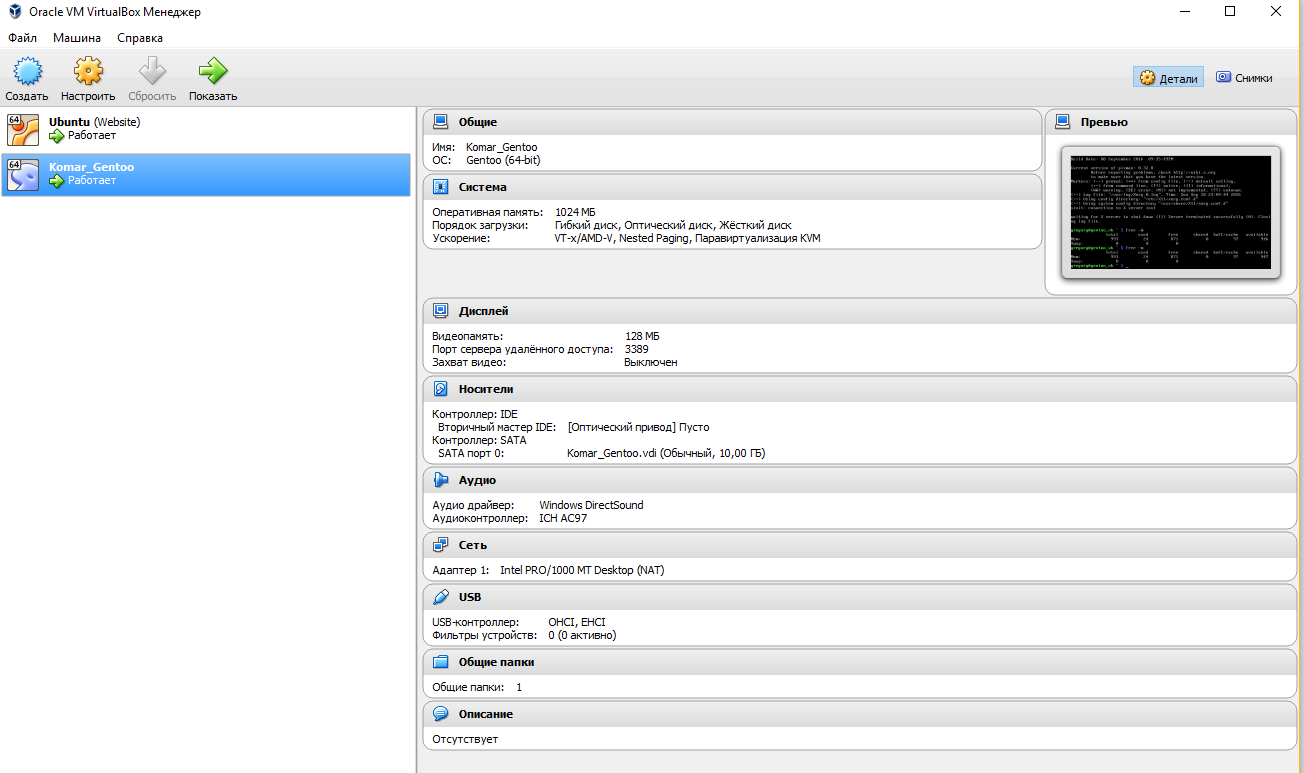
\includegraphics[width=\textwidth]{q3screen.png}
	\caption{Знімок головного екрану ВМ із відображенням параметрів ВМ}
\end{figure}

\section{Відповіді на п.5 та п.6}
На хостовій ОС «Windows 10» VirtualBox створює в директорії користувача 
директорію «VirtualBox VMs». Кожна віртуальна машина має в ній окрему субдиректорію, в якій містяться:
\begin{itemize}
	\item XML файли з конфігурацією віртуальної машини, які мають розширення 
	.vbox та їх бекапи з розширенням .vbox-prev
	\item За замовчуванням тут знаходяться файли віртуальних дисків 
	гостьових ОС
	\item Директорія Logs логами роботи віртуальної машини
	\item Директорія Snapshots
\end{itemize}
Після створення знімку стану ОС в директорії Snapshots з'явився файл
диференціального жорсткого диску та файл з розширенням .sav, назва
якого містила поточну дату та час.
Після збереження стану в директорії Snapshots з'явився ще один файл з
розширенням .sav.
Варто зазначити, що при модифікації файлів в файловій системі гостьової
ОС розмір файлів диференціальних дисків змінювався.
Експорт віртуальної машини виконувався протягом  досить тривалого часу,
значно більшого ніж збереження стану та створення снапшотів. Результатом
експорту став  файл з розширенням .ova, який можна використати для 
перенесення віртуальної машини на інші хостові системи.

VirtualBox дозволяє користувачу зробити спільним буфер обміну між хостовою ОС
та гостьовою ОС. Це дозволяє передавати в ОС такі данні як веб-посилання та
файли конфігурації і при цьому уникнути помилок при введенні цих данних 
вручну а також зекономити час. Однак використання спільного буфера можна
уникнути при взаємодії з гостьовою ОС засобами SSH та використанні мережевої
прозорості протоколу X. Для використання буфера обміну потрібно 
встановити спеціальне програмне забезпечення на гостьову ОС. Функція 
Drag'n'Drop не запрацювала, можливою причиною чого стала різноманітність
ОС на ядрі Linux, і неможливість створення стандартної реалізації цієї
функції. Однак для передачі файлів між хостом та гостем можна
використовувати спільні директорії.
\section{Висновки}
Під час виконання лабораторної роботи я ознайомився з принципами роботи
віртуальних машин на прикладі системи віртуалізації VirtualBox.
Мною була створена і налаштована віртуальна машина з гостьовою ОС 
Gentoo. Я використовував функції створення знімків стану гостьової ОС та
експорту віртуальної машини.
\end{document}
